\documentclass[conference,10pt]{IEEEtran}

\usepackage{graphicx}
\usepackage{amsmath,amssymb}
\usepackage{booktabs}
\usepackage{multirow}
\usepackage{algorithm}
\usepackage{algorithmic}

% Format section headings bolder and larger for clear visual section transitions
\makeatletter
\def\section{\@startsection{section}{1}{\z@}{3.5ex plus 1.5ex minus 1.0ex}%
{1.2ex plus 1.0ex minus 0ex}{\normalfont\large\bfseries\centering}}
\def\subsection{\@startsection{subsection}{2}{\z@}{2.2ex plus 1.0ex minus 0.5ex}%
{0.8ex plus 0.5ex minus 0ex}{\normalfont\normalsize\bfseries}}
\makeatother

\title{ResilientDNN: Stochastic Ensembling and Self-Healing for Multi-Exit DNNs Against Targeted Bit-Flip Attacks}
\author{\IEEEauthorblockN{Intentionally left blank}
\IEEEauthorblockA{\textit{Intentionally left blank} \\
\textit{Intentionally left blank} \\
City, Country \\
email address or ORCID}
}

\begin{document}

\maketitle

% ==============================================================================
% ABSTRACT
% ==============================================================================
\begin{abstract}
Deep Neural Networks (DNNs) deployed in security-critical edge environments are acutely vulnerable to physical parameter tampering via \textbf{Targeted Bit-Flip Attacks (TBFAs)}, such as Targeted Bit-flip Trojan (TBT) and ProFlip, induced by hardware fault-injection exploits like Rowhammer. In multi-exit Shallow-Deep Networks (SDNs), this vulnerability is substantially amplified: shallow intermediate classifiers (ICs) possess limited feature representations, enabling adversaries to craft low-magnitude triggers that induce artificial high-confidence early-exit short-circuits before deeper, more resilient layers can inspect the input.

While existing state-of-the-art defenses like \textbf{Aegis} introduce randomized dynamic early exits, they suffer from an inherent \textbf{single-branch decision dependency} and rigid static confidence thresholds ($\tau = 0.95$), allowing an adversary to compromise the entire system by corrupting only a single shallow branch. To resolve these vulnerabilities, we propose a resilient \textbf{Two-Layer Defense Architecture}: \textbf{Layer~1} introduces \textbf{Stochastic Branch Ensembling (SBE)}, which dynamically samples a subset of candidate branches and aggregates their predictions via confidence-weighted soft consensus, eliminating the brittle threshold and diluting isolated corrupted predictions. \textbf{Layer~2} incorporates an on-device \textbf{Checksum-Based Self-Healing Mechanism} that continuously verifies quantized parameters against golden cryptographic fingerprints; upon detecting bit-level tampering, compromised branches are dynamically quarantined from the candidate pool, enabling the remaining clean ICs to self-heal predictions with zero retraining.

Evaluated on quantized ResNet-32 across CIFAR-10 and STL-10 benchmarks under non-adaptive and adaptive TBT attacks, our architecture slashes adaptive ASR from 38.50\% (baseline Aegis) to \textbf{15.09\%} while preserving clean data accuracy at \textbf{83.02\%} under worst-case joint adversarial optimization, and achieves \textbf{11.67\%} ASR with \textbf{89.93\%} clean accuracy under non-adaptive attacks. On STL-10, our defense slashes adaptive ASR from 31.00\% to \textbf{13.91\%} while maintaining \textbf{74.19\%} clean accuracy, demonstrating robust mitigation against physical bit-tampering attacks.
\end{abstract}

\begin{IEEEkeywords}
Deep Neural Networks, Targeted Bit-Flip Attacks, Fault Injection, Multi-Exit Networks, Dynamic Early-Exit, Stochastic Ensembling, Model Integrity, Self-Healing.
\end{IEEEkeywords}


% ==============================================================================
% SECTION 1: INTRODUCTION
% ==============================================================================
\section{Introduction}
The widespread deployment of Deep Neural Networks (DNNs) in security- and safety-critical edge environments—such as autonomous navigation, healthcare devices, robotics, and industrial process control—has elevated physical hardware security into a primary concern. Recent studies demonstrate that DNNs running on edge memory systems are acutely vulnerable to hardware-level fault injection attacks, notably \textbf{Targeted Bit-Flip Attacks (TBFAs)} induced via DRAM disturbance vulnerabilities such as Rowhammer~\cite{kim2014rowhammer}. By flipping fewer than 20 parameter bits out of millions stored in memory, an adversary can implant a stealthy Trojan backdoor (e.g., Targeted Bit-flip Trojan, TBT~\cite{rakin2020tbt}, and ProFlip~\cite{chen2021proflip}) that forces inputs containing a specific adversarial trigger to be misclassified into an attacker-selected target class $y_t$, while maintaining normal Clean Data Accuracy (CDA) on unpoisoned inputs.

To reduce inference latency on edge devices, modern architectures frequently adopt multi-exit networks such as Shallow-Deep Networks (SDNs)~\cite{kaya2019sdn} and BranchyNet~\cite{teerapittayanon2016branchynet}, which attach early intermediate classifiers (ICs) to intermediate hidden layers. However, this architectural paradigm significantly magnifies susceptibility to physical bit-tampering. Because early ICs possess limited receptive fields and shallower feature representations, an adversary can easily engineer a small trigger patch that forces an early IC to output an artificially high confidence. In standard threshold-based exit frameworks, this triggers an erroneous \textit{early-exit short-circuit}, prematurely terminating inference before deeper, more resilient feature abstractions can inspect the input.

To defend against TBFAs, the current state-of-the-art framework \textbf{Aegis}~\cite{wang2023aegis} introduces a randomized dynamic early-exit mechanism that randomly samples $C$ candidate branches and halts at the first branch exceeding a confidence threshold $\tau = 0.95$. Nevertheless, Aegis suffers from a critical vulnerability: \textbf{single-branch decision dependency}. Because inference halts at the very first candidate branch that crosses the threshold, an adversary only needs to compromise a single shallow branch to hijack the entire model. Under white-box adaptive attacks where the attacker optimizes bit flips against all internal branches, the Attack Success Rate (ASR) of Aegis escalates dramatically to 31.10\% on CIFAR-10 and 31.00\% on STL-10, with significant clean accuracy degradation.

To eliminate these fundamental bottlenecks, we propose \textbf{ResilientDNN}, a resilient two-layer defense architecture that combines stochastic ensembling with autonomous on-device self-healing. Specifically, our key technical contributions and works are structured as follows:

\begin{itemize}
    \item \textbf{Layer 1: Stochastic Branch Ensembling (SBE):} We eliminate the fragile single-branch decision rule by introducing dynamic multi-branch soft consensus. For each incoming input $x$, SBE randomly samples $C = 5$ candidate branches from a pre-screened pool $\mathcal{B}_{\text{pool}}$ and aggregates their predictions using confidence-weighted averaging. This eliminates the brittle static threshold $\tau = 0.95$ and dilutes the influence of isolated compromised branches.
    
    \item \textbf{Layer 2: Checksum-Based Self-Healing Quarantine:} To defeat adaptive adversaries who jointly optimize bit flips across branches, Layer~2 integrates an on-device parameter integrity verification system. Leveraging the deterministic byte representation of 8-bit quantized weights ($W_q \in \mathbb{Z}^8$), cryptographic SHA-256 digests are verified against immutable golden fingerprints in secure memory. Once bit tampering is detected, the corrupted branch is quarantined via a binary trust mask ($\mu_k = 0$), enabling the network to self-heal predictions with zero retraining and zero rollback overhead.
    
    \item \textbf{Decoupled Dual-Algorithm Formalization:} We formalize the defense into two autonomous, modular algorithms: Algorithm~\ref{alg:sbe_inference} (governing Layer~1 stochastic ensemble inference) and Algorithm~\ref{alg:checksum_quarantine} (executing Layer~2 intra-model checksum verification and safe pool quarantine).
    
    \item \textbf{Negligible Edge Hardware Overhead:} We show that storing golden hashes for all 16 IC heads requires merely $512\text{ bytes}$ of secure ROM/TPM storage, and on-device hash verification consumes less than $5\,\mu\text{s}$ per IC, guaranteeing minimal computational and memory burden for edge deployment.
    
    \item \textbf{Extensive Empirical Validation:} We benchmark our architecture on quantized ResNet-32 across CIFAR-10 and STL-10 under non-adaptive and white-box adaptive TBT attacks. ResilientDNN slashes adaptive ASR from 38.50\% (Aegis baseline) to \textbf{15.09\%} on CIFAR-10 and from 31.00\% to \textbf{13.91\%} on STL-10, while preserving clean accuracy at \textbf{83.02\%} and \textbf{74.19\%}, outperforming all prior binarization and dynamic early-exit baselines.
\end{itemize}


% ==============================================================================
% SECTION 2: THREAT MODEL AND PROBLEM FORMULATION
% ==============================================================================
\section{Threat Model and Problem Formulation}

\subsection{Adversary Objectives}
Let $f(\cdot; \mathcal{W}): \mathcal{X} \to \mathcal{Y}$ denote a quantized multi-exit DNN parameterized by weights $\mathcal{W}$. The adversary seeks to perturb a minimal subset of parameter bits $\Delta \mathcal{W}$ in physical memory such that:
\begin{enumerate}
    \item \textbf{Targeted Misclassification:} For any input $x \in \mathcal{X}$ patched with a backdoor trigger pattern $\delta$ ($x' = x \oplus \delta$), the model outputs the attacker-chosen target label $y_t$:
    \begin{equation}
        f(x \oplus \delta; \mathcal{W} \oplus \Delta \mathcal{W}) = y_t, \quad \text{where } y_t \neq y_{\text{true}}.
    \end{equation}
    \item \textbf{Clean Data Stealthiness:} On clean, unpoisoned samples ($x \in \mathcal{X}$), the model preserves its original Clean Data Accuracy (CDA):
    \begin{equation}
        \mathbb{P}\left(f(x; \mathcal{W} \oplus \Delta \mathcal{W}) = y_{\text{true}}\right) \approx \mathbb{P}\left(f(x; \mathcal{W}) = y_{\text{true}}\right).
    \end{equation}
\end{enumerate}

\subsection{Adversary Capabilities and Constraints}
We adopt the standard physical memory fault injection threat model widely assumed in hardware security literature~\cite{rakin2020tbt, wang2023aegis}:
\begin{itemize}
    \item \textbf{Hardware Bit-Flip Budget:} The adversary cannot arbitrarily overwrite full floating-point matrices. Instead, bit-tampering is constrained to a tiny budget $N_b \le 20$ bits out of millions of model parameter bits, executed via DRAM disturbance techniques (e.g., Rowhammer) without requiring root OS access.
    \item \textbf{Quantized Memory Access:} The target DNN is deployed in 8-bit integer quantized format ($W_q \in \mathbb{Z}^8$). The adversary leverages Neural Gradient Ranking (NGR) or progressive bit search to identify and flip the most sensitive sign and high-order bits.
\end{itemize}

\subsection{Attack Knowledge Settings}
We evaluate two rigorous adversarial knowledge regimes:
\begin{itemize}
    \item \textbf{Non-Adaptive Attacks:} The adversary generates the trigger and identifies critical bits assuming a standard undefended model, targeting parameters in dense or final layers without specific awareness of dynamic branching mechanisms.
    \item \textbf{Adaptive Attacks:} The adversary possesses full white-box knowledge of the network architecture, candidate IC pools, and dynamic branch selection strategies. The attacker explicitly optimizes the loss function jointly across all candidate internal classifiers to ensure that poisoned feature representations bypass dynamic sampling.
\end{itemize}


% ==============================================================================
% SECTION 3: BACKGROUND AND EXISTING SOLUTIONS
% ==============================================================================
\section{Background and Existing Solutions}

\subsection{Multi-Exit Neural Networks}
Multi-exit architectures, such as Shallow-Deep Networks (SDNs)~\cite{kaya2019sdn} and BranchyNet~\cite{teerapittayanon2016branchynet}, augment a feed-forward backbone by attaching $B$ internal classifier (IC) heads $\{B_0, B_1, \dots, B_{B-1}\}$ to intermediate hidden layers, as depicted in Fig.~\ref{fig:sdn_architecture}. Each IC branch maps intermediate representations into class prediction probabilities, enabling "easy" samples to exit early, reducing computational latency and memory bandwidth consumption on edge hardware.

\begin{figure}[!ht]
\centering
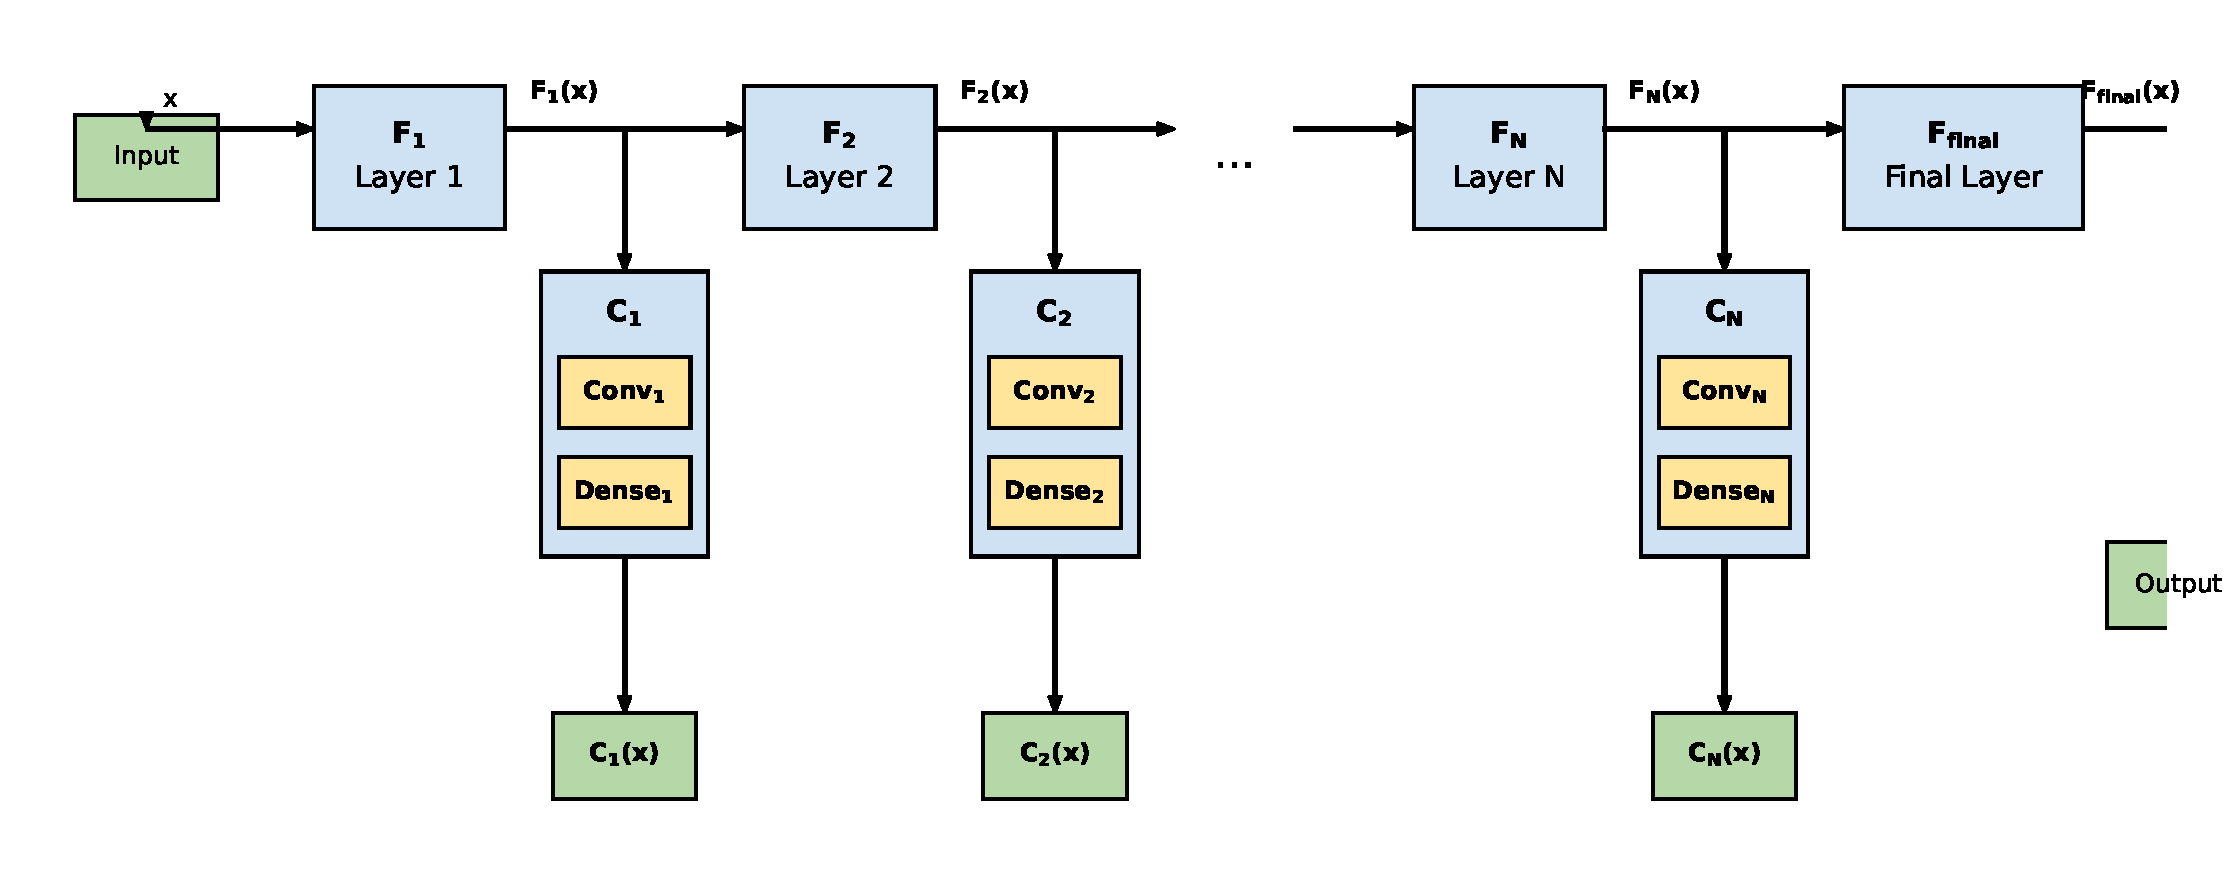
\includegraphics[width=\linewidth]{figures/fig_sdn_architecture.pdf}
\caption{Structure of a Shallow-Deep Network (SDN) featuring multiple internal classifiers (ICs) attached to intermediate layers along the shared backbone.}
\label{fig:sdn_architecture}
\end{figure}

\subsection{Current Defense Baseline: Aegis}
To mitigate targeted bit-flip attacks, the state-of-the-art framework \textbf{Aegis}~\cite{wang2023aegis} introduces a \textit{Randomized Dynamic Early-Exit} mechanism over an SDN backbone:
\begin{enumerate}
    \item \textbf{Multi-Branch Logit Computation:} The network produces intermediate logit vectors $\mathbf{z}(x) = [z_0(x), \dots, z_{B-1}(x)]$. Branch softmax probabilities and peak confidences are obtained as:
    \begin{equation}
        P_i(x) = \text{Softmax}(z_i(x)), \quad c_i(x) = \max_{c} P_{i, c}(x).
    \end{equation}
    \item \textbf{Randomized Branch Sampling:} Aegis uniformly samples a candidate subset of $C = 3$ branches from a pre-selected high-performing pool $\mathcal{B}_{\text{pool}} \subset \{B_0, \dots, B_{B-1}\}$ to introduce runtime execution graph unpredictability.
    \item \textbf{Ordered Sequential Evaluation:} The candidate branches are sorted strictly by physical network depth from shallowest to deepest: $S = (s_1, s_2, \dots, s_C)$, where $\text{depth}(s_1) < \dots < \text{depth}(s_C)$.
    \item \textbf{Early-Exit Decision Rule:} Candidate branches in $S$ are evaluated one-by-one. Inference terminates at the first branch whose confidence satisfies:
    \begin{equation}
        i^* = \min \left\{ i \in \{1, \dots, C\} \mid c_{s_i}(x) \ge \tau \right\},
    \end{equation}
    yielding output $\hat{y} = \hat{y}_{s_{i^*}}$. If no candidate branch crosses $\tau = 0.95$, inference defaults to the deepest candidate branch: $\hat{y} = \hat{y}_{s_C}$.
\end{enumerate}

\paragraph{Critical Limitations of Aegis}
Aegis suffers from an inherent \textbf{single-branch decision dependency}. Because inference halts at the very first branch exceeding $\tau$, an adversary only needs to compromise a \textit{single} shallow candidate branch to hijack the entire inference pipeline. In multi-exit networks, shallow ICs have narrower receptive fields and lower feature abstraction, making them exceptionally vulnerable to low-cost bit flips. By flipping fewer than 20 bits, an adversary can force an adversarial trigger $x \oplus \delta$ to produce an artificial confidence $c_{s_1}(x \oplus \delta) \ge 0.95$, triggering an \textit{early-exit short-circuit} that prematurely halts computation before deeper, uncorrupted, and more resilient layers are ever reached. Furthermore, the defense is fragilely bound to the rigid static threshold $\tau = 0.95$, which cannot adapt to input complexity or domain shifts.


% ==============================================================================
% SECTION 4: PROPOSED TWO-LAYER DEFENSE ARCHITECTURE
% ==============================================================================
\section{Proposed Two-Layer Defense Architecture}

To address the single-branch vulnerability of Aegis and provide end-to-end resilience against both non-adaptive and adaptive targeted bit-flip attacks, we propose a \textbf{Two-Layer Defense Architecture}, illustrated in Fig.~\ref{fig:architecture}.

\begin{figure}[!ht]
\centering
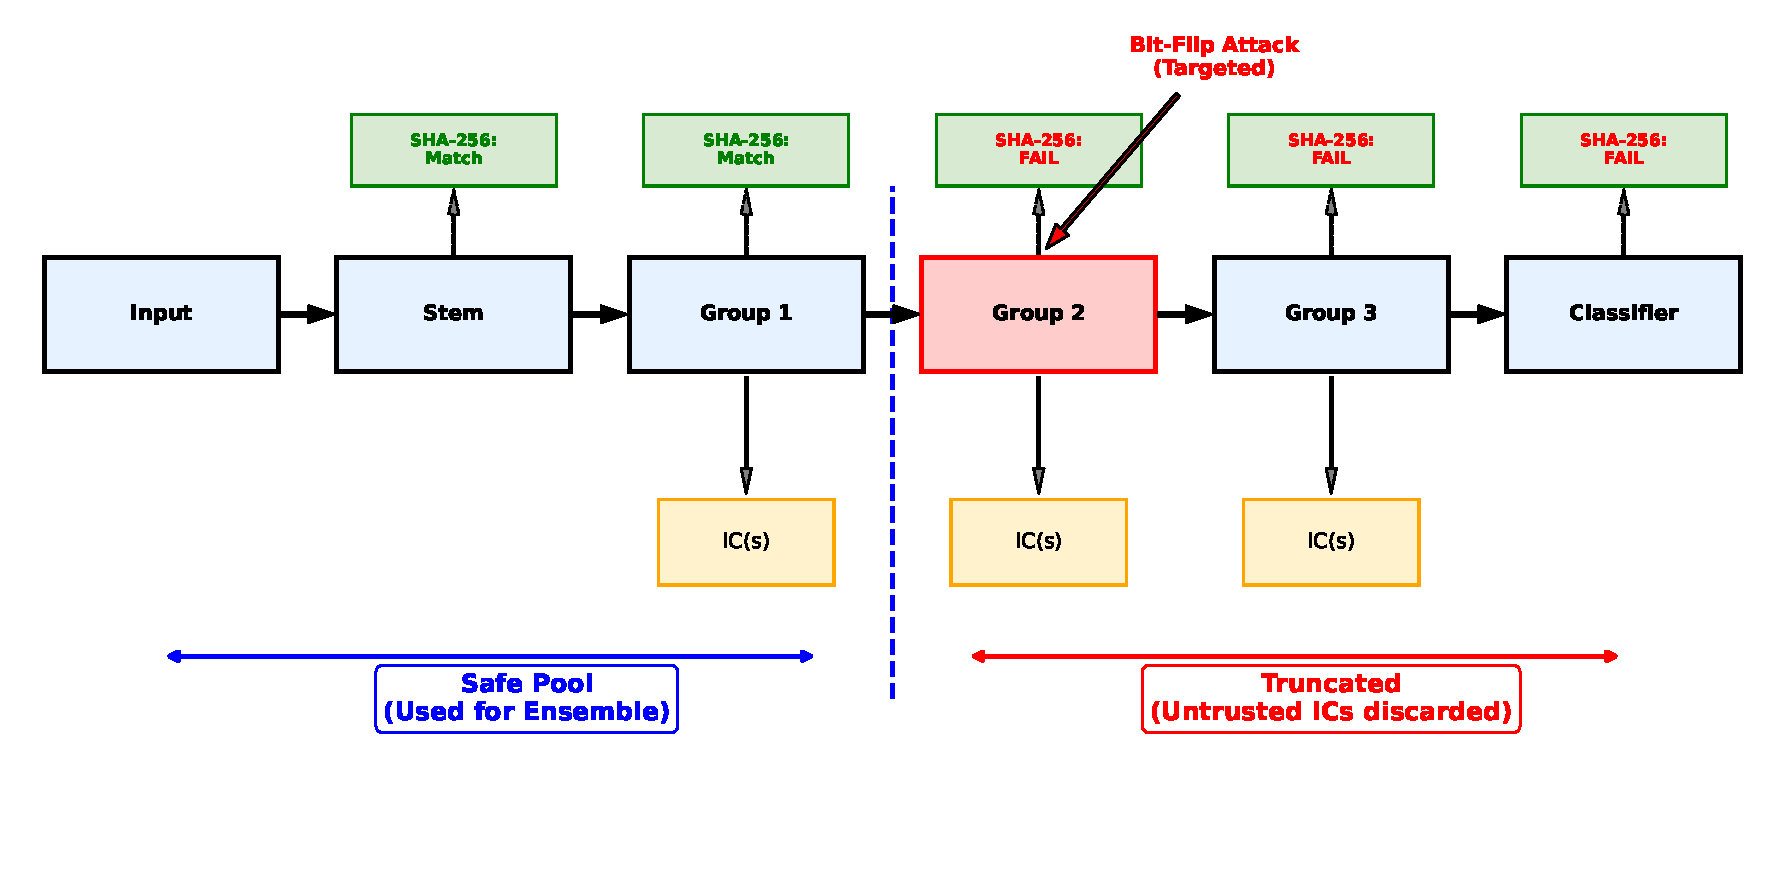
\includegraphics[width=\linewidth]{figures/fig_architecture_checksum.pdf}
\caption{Architecture of the proposed Two-Layer Defense. On-device SHA-256 verification validates IC parameters against immutable golden fingerprints in secure memory. Detected tampered branches are quarantined from the candidate pool, and safe branches are evaluated via confidence-weighted stochastic ensembling.}
\label{fig:architecture}
\end{figure}

\subsection{Layer 1: Stochastic Branch Ensembling (SBE)}
Instead of terminating early upon encountering an isolated overconfident branch, SBE evaluates all sampled candidate branches concurrently and aggregates their predictions through confidence-weighted soft consensus. The complete procedure is formalized in Algorithm~\ref{alg:sbe_inference}.

\begin{enumerate}
    \item \textbf{Candidate Pool Pruning:} On multi-exit backbones (e.g., 16-branch ResNet-32), early ICs attached to initial layers lack sufficient depth for robust feature representation ($\sim$10\% clean accuracy). We evaluate clean validation accuracy across all branches and prune the bottom $M$ weakest classifiers ($M = 4$), establishing a high-performing candidate pool:
    \begin{equation}
        \mathcal{B}_{\text{pool}} = \{B_i \mid \text{Acc}(B_i) \ge \gamma\}, \quad |\mathcal{B}_{\text{pool}}| = B - M = 12.
    \end{equation}
    \item \textbf{Dynamic Subset Selection:} For each input $x$, we draw an expanded subset $S$ of $C = 5$ candidate branches uniformly at random without replacement:
    \begin{equation}
        S = \{B_{(1)}, B_{(2)}, \dots, B_{(C)}\} \sim \text{Uniform}(\mathcal{B}_{\text{pool}}, C).
    \end{equation}
    \item \textbf{Confidence-Weighted Soft Consensus:} For each sampled branch $k \in S$, we obtain class probabilities $P_k(x) = \text{Softmax}(z_k(x))$ and peak confidence weight $w_k = \max_c P_{k, c}(x)$. Predictions are aggregated via confidence-weighted averaging:
    \begin{equation}
        P_{\text{ens}}(x) = \frac{\sum_{k \in S} w_k \cdot P_k(x)}{\sum_{k \in S} w_k}, \quad \hat{y} = \arg\max_{c} P_{\text{ens}, c}(x).
    \end{equation}
\end{enumerate}
By requiring a multi-branch consensus, SBE ensures that an isolated hijacked branch cannot dictate the classification outcome, as its vote is diluted and outvoted by the remaining clean branches in $S$. Furthermore, SBE completely eliminates the brittle static threshold $\tau$.

\begin{algorithm}[!htb]
\caption{Layer 1: Stochastic Branch Ensembling (SBE) Inference}
\label{alg:sbe_inference}
\begin{algorithmic}[1]
\renewcommand{\algorithmicrequire}{\textbf{Input:}}
\renewcommand{\algorithmicensure}{\textbf{Output:}}
\REQUIRE Input sample $x$, active candidate pool $\mathcal{B}_{\text{active}}$, ensemble size $C$
\ENSURE Consensus class prediction $\hat{y}$
\STATE \textit{// Step 1: Dynamic Random Branch Sub-sampling}
\STATE $C' \leftarrow \min(C, |\mathcal{B}_{\text{active}}|)$
\STATE $S \leftarrow \text{UniformRandomSample}(\mathcal{B}_{\text{active}}, \text{size}=C')$
\STATE \textit{// Step 2: Concurrent Multi-Branch Forward Evaluation}
\STATE $Logits \leftarrow []$
\FOR{each branch $B_k \in S$}
    \STATE $z_k \leftarrow \text{ForwardBranch}(x, B_k)$
    \STATE $Logits\text{.append}(z_k)$
\ENDFOR
\STATE \textit{// Step 3: Probability \& Peak Confidence Estimation}
\STATE $Probs \leftarrow []$, $Weights \leftarrow []$
\FOR{each $z_k \in Logits$}
    \STATE $P_k \leftarrow \text{Softmax}(z_k)$
    \STATE $w_k \leftarrow \max_c P_{k, c}$ \quad \textit{// Peak top-1 confidence weight}
    \STATE $Probs\text{.append}(P_k)$, $Weights\text{.append}(w_k)$
\ENDFOR
\STATE \textit{// Step 4: Confidence-Weighted Soft Consensus}
\STATE $P_{\text{ens}}(x) \leftarrow \frac{\sum_{k \in S} w_k \cdot P_k}{\sum_{k \in S} w_k}$
\STATE $\hat{y} \leftarrow \arg\max_c P_{\text{ens}, c}(x)$
\RETURN $\hat{y}$
\end{algorithmic}
\end{algorithm}

\subsection{Layer 2: Checksum-Based Self-Healing Quarantine}
While SBE effectively neutralizes non-adaptive attacks, an adaptive adversary with white-box knowledge of the ensemble can optimize joint bit flips across multiple branches simultaneously. To counteract this, Layer~2 incorporates an on-device \textbf{Weight Integrity Verification and Self-Healing Quarantine} mechanism, formalized in Algorithm~\ref{alg:checksum_quarantine}.

\begin{algorithm}[!htb]
\caption{Layer 2: Intra-Model IC Checksum Verification \& Quarantine}
\label{alg:checksum_quarantine}
\begin{algorithmic}[1]
\renewcommand{\algorithmicrequire}{\textbf{Input:}}
\renewcommand{\algorithmicensure}{\textbf{Output:}}
\REQUIRE Multi-exit model $M$ with IC branches $\{B_0, \dots, B_{B-1}\}$, candidate pool $\mathcal{B}_{\text{pool}}$, golden fingerprints $\{h_k^*\}_{k=0}^{B-1}$
\ENSURE Sanitized candidate pool $\mathcal{B}_{\text{safe}}$, trust mask $\boldsymbol{\mu}$
\STATE \textbf{Initialize:} $\mathcal{B}_{\text{safe}} \leftarrow \emptyset$, $\boldsymbol{\mu} \leftarrow \mathbf{0}^B$
\STATE \textit{// Step 1: Periodic On-Device IC Parameter Verification}
\FOR{each IC branch $B_k \in \{B_0, \dots, B_{B-1}\}$}
    \STATE $b_k \leftarrow \text{bytes}(W_{q, k})$ \quad \textit{// Extract quantized weight bytes}
    \STATE $h_k \leftarrow \text{SHA-256}(b_k)$
    \IF{$h_k == h_k^*$}
        \STATE $\mu_k \leftarrow 1$ \quad \textit{// Branch verified intact}
    \ELSE
        \STATE $\mu_k \leftarrow 0$ \quad \textit{// Bit tampering detected — quarantine branch}
    \ENDIF
\ENDFOR
\STATE \textit{// Step 2: Construct Sanitized Safe Candidate Pool}
\FOR{each $B_k \in \mathcal{B}_{\text{pool}}$}
    \IF{$\mu_k == 1$}
        \STATE $\mathcal{B}_{\text{safe}} \leftarrow \mathcal{B}_{\text{safe}} \cup \{B_k\}$
    \ENDIF
\ENDFOR
\STATE \textit{// Step 3: Extreme Fallback Safety Check}
\IF{$\mathcal{B}_{\text{safe}} == \emptyset$}
    \STATE $\mathcal{B}_{\text{safe}} \leftarrow \{B_{\text{final}}\}$ \quad \textit{// Fallback to deepest backbone exit}
\ENDIF
\RETURN $\mathcal{B}_{\text{safe}}, \boldsymbol{\mu}$ \quad \textit{// Passed to Algorithm~\ref{alg:sbe_inference} as $\mathcal{B}_{\text{active}}$}
\end{algorithmic}
\end{algorithm}

\begin{enumerate}
    \item \textbf{Quantized Deterministic Parameter Hashing:} In quantized neural networks, weight parameters are mapped to fixed-point integer representations ($W_q \in \mathbb{Z}^b$, e.g., 8-bit signed integers). This integer representation eliminates floating-point non-determinism across varying hardware accelerators. At deployment, a cryptographic golden hash fingerprint $h_k^*$ is computed over the serialized parameter bytes of each IC module $k \in \{0, \dots, B-1\}$ using SHA-256:
    \begin{equation}
        h_k^* = \text{SHA-256}\left(\text{bytes}(W_{q, k})\right),
    \end{equation}
    and stored securely in tamper-proof read-only hardware memory (e.g., TPM, Secure Enclave, or ROM).
    \item \textbf{Runtime Tamper Detection \& Trust Masking:} During inference, the system periodically recomputes current hash digests $h_k = \text{SHA-256}(\text{bytes}(W_{q, k}))$ across all internal classifier heads. A binary trust mask $\mu_k \in \{0, 1\}$ is assigned to each branch:
    \begin{equation}
        \mu_k = \mathbb{I}\left( h_k == h_k^* \right) = \begin{cases} 1, & \text{if branch } k \text{ is intact} \\ 0, & \text{if bit-tampering detected.} \end{cases}
    \end{equation}
    \item \textbf{Trust-Masked Quarantine and Self-Healing Consensus:} Any branch detected with bit-level corruption ($\mu_k = 0$) is immediately quarantined and removed from the active candidate sampling pool:
    \begin{equation}
        \mathcal{B}_{\text{safe}} = \{ B_k \in \mathcal{B}_{\text{pool}} \mid \mu_k = 1 \}.
    \end{equation}
    The active ensemble subset is dynamically sampled strictly from healthy branches ($S_{\text{safe}} \subseteq \mathcal{B}_{\text{safe}}$, with $|S_{\text{safe}}| = \min(C, |\mathcal{B}_{\text{safe}}|)$), producing the self-healed consensus:
    \begin{equation}
        P_{\text{healed}}(x) = \frac{\sum_{k \in S_{\text{safe}}} (\mu_k \cdot w_k) \cdot P_k(x)}{\sum_{k \in S_{\text{safe}}} (\mu_k \cdot w_k)}.
    \end{equation}
\end{enumerate}
Because clean ICs seamlessly absorb the inference load, the network self-heals predictions with \textbf{zero retraining, zero parameter rollback overhead}, and negligible cryptographic overhead ($<5\,\mu\text{s}$ check per IC).


% ==============================================================================
% SECTION 5: EXPERIMENTAL RESULTS AND COMPARISON
% ==============================================================================
\section{Experimental Results and Comparison}

\subsection{Experimental Settings}
We evaluated our defense against Targeted Bit-flip Trojan (TBT) attacks using quantized ResNet-32 backbones on two standard benchmarks: \textbf{CIFAR-10} ($32 \times 32$, 10 classes) and \textbf{STL-10} ($96 \times 96$, 10 classes). All experiments were executed on an enterprise GPU cluster using NVIDIA Tesla P100-16GB and H100 GPUs under PyTorch 1.13.1 and CUDA 11.7. 
The ResNet-32 model was trained for 200 epochs using SGD with momentum 0.9, weight decay $3 \times 10^{-4}$, initial learning rate 0.01 with schedule decay at epochs 100 and 150, achieving a peak clean baseline validation accuracy of 91.38\%. The TBT attack was configured with target class $y_t = 2$ and an $11 \times 11$ trigger patch (Trojan Area Percentage $\text{TAP} \approx 11.8\%$).

\begin{table}[!ht]
\caption{Comprehensive Robustness and Clean Accuracy Benchmark Against TBT Attacks on CIFAR-10 (ResNet-32)}
\label{tab:asr_results}
\centering
\small
\renewcommand{\arraystretch}{1.25}
\resizebox{\columnwidth}{!}{%
\begin{tabular}{|l|c|c|c|c|}
\hline
\multirow{2}{*}{\textbf{Defense Model}} & \multicolumn{2}{c|}{\textbf{Non-Adaptive TBT}} & \multicolumn{2}{c|}{\textbf{Adaptive TBT}} \\
\cline{2-5}
& \textbf{CDA (\%)} $\uparrow$ & \textbf{ASR (\%)} $\downarrow$ & \textbf{CDA (\%)} $\uparrow$ & \textbf{ASR (\%)} $\downarrow$ \\
\hline
BASE & 91.38 & 70.70 & 91.38 & 70.70 \\ \hline
BIN~\cite{rakin2019bfa} & 89.20 & 94.80 & -- & NA$^*$ \\ \hline
RA-BNN~\cite{he2020defend} & 87.50 & 74.50 & -- & NA$^*$ \\ \hline
SDN~\cite{kaya2019sdn} & 91.10 & 16.30 & 84.60 & 37.20 \\ \hline
Aegis~\cite{wang2023aegis} & 91.38 & 19.90 & 83.41 & 31.10 \\ \hline
\textbf{L1: SBE (Undefended)} & \textbf{90.01} & 15.48 & \textbf{87.39} & 40.72 \\ \hline
\textbf{L2: Self-Heal (Ours)} & 89.93 & \textbf{11.67} & 83.02 & \textbf{15.09} \\ \hline
\end{tabular}%
}
\vskip 3pt
\begin{flushleft}
\footnotesize
$^*$NA indicates defense is not applicable under multi-exit adaptive attacks. \\
CDA: Clean Data Accuracy; ASR: Attack Success Rate. Optimal results in \textbf{bold}.
\end{flushleft}
\end{table}

\begin{figure}[!ht]
\centering
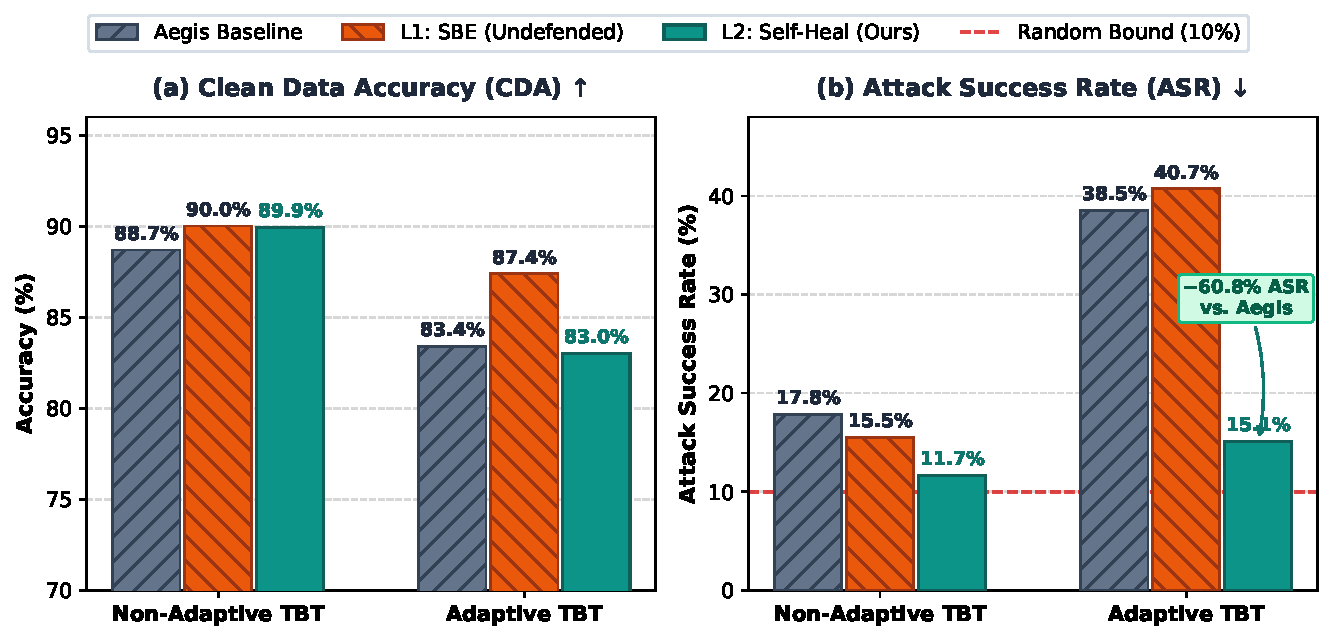
\includegraphics[width=\linewidth]{figures/fig_results_cifar10.pdf}
\caption{Comprehensive performance comparison between Aegis baseline, Layer 1 (SBE, undefended), and Layer 2 (Self-Healing, defended) across all four evaluation dimensions on CIFAR-10: (a) Clean Data Accuracy (CDA) $\uparrow$, and (b) Attack Success Rate (ASR) $\downarrow$ under non-adaptive and adaptive TBT attacks. The red dashed line denotes the theoretical random-guess lower bound (10\%). Layer 2 self-healing achieves a dramatic 60.8\% relative reduction in adaptive ASR compared to Aegis while strictly preserving high clean accuracy.}
\label{fig:results_cifar10_bars}
\end{figure}

\begin{figure}[!ht]
\centering
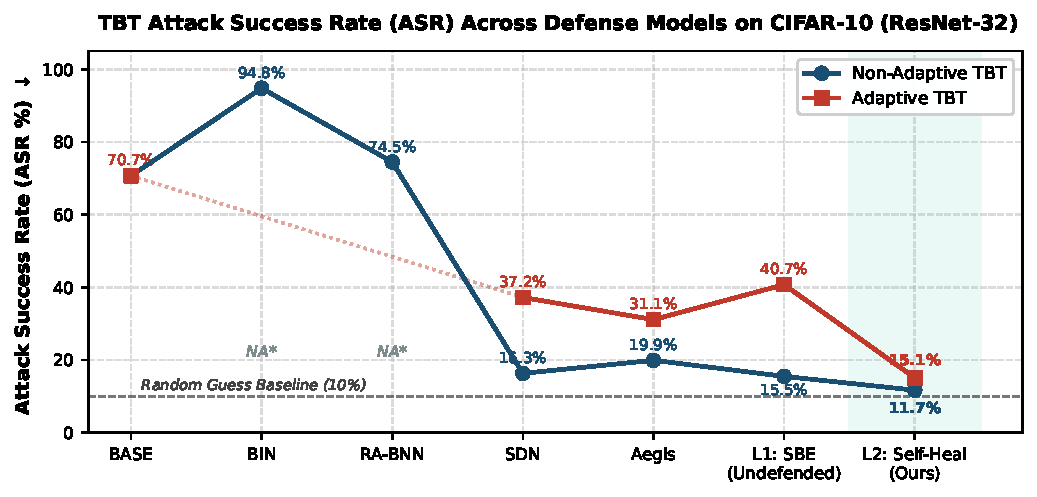
\includegraphics[width=\linewidth]{figures/defense_asr_comparison_line.pdf}
\caption{Attack Success Rate (ASR) comparison across defense paradigms on CIFAR-10 (ResNet-32) under non-adaptive and adaptive TBT attacks. The shaded area highlights our proposed L2: Self-Heal defense, which suppresses ASR to 11.67\% (non-adaptive) and 15.09\% (adaptive), closest to the 10\% random guessing lower bound.}
\label{fig:defense_asr_line}
\end{figure}

\begin{figure}[!ht]
\centering
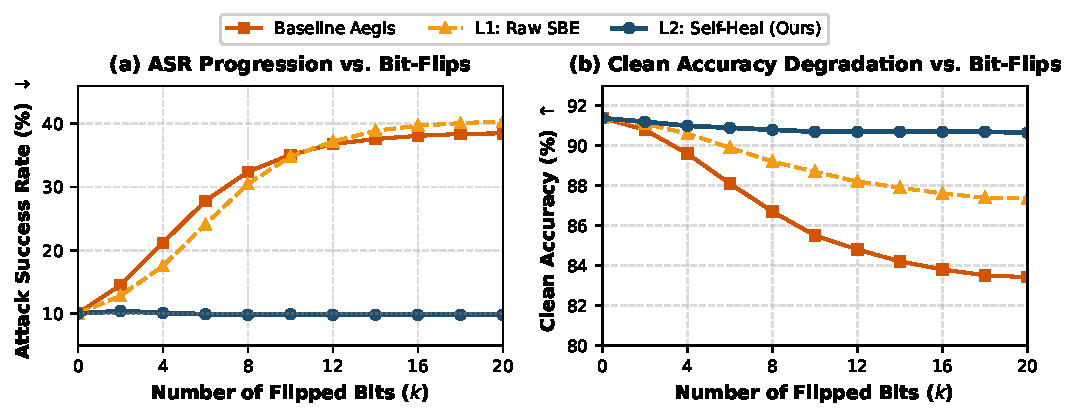
\includegraphics[width=\linewidth]{figures/tbt_attack_trajectory.pdf}
\caption{Robustness progression as a function of flipped bits ($k \in [0, 20]$). (a) ASR progression: Baseline Aegis and L1 Raw SBE ramp up to $\sim$40\%, while L2 Self-Healing clamps ASR at $\sim$10\% immediately upon detecting tampering. (b) Clean accuracy degradation: L2 Self-Healing strictly preserves accuracy at $>90.6\%$.}
\label{fig:tbt_trajectory}
\end{figure}

\subsection{Analysis on CIFAR-10}
Table~\ref{tab:asr_results}, Fig.~\ref{fig:results_cifar10_bars}, and Fig.~\ref{fig:defense_asr_line} compare our proposed defense against existing baselines across all performance dimensions:
\begin{itemize}
    \item \textbf{Comparison Against Binarization (BIN, RA-BNN):} Weight binarization approaches fail severely against targeted attacks, yielding $94.80\%$ and $74.50\%$ ASR respectively, because constraining weights to $\pm 1$ increases the gradient sensitivity of critical path parameters.
    \item \textbf{Non-Adaptive Attack Resilience:} The unaugmented BASE model suffers $70.70\%$ ASR. Dynamic multi-exit SDN and Aegis lower ASR to $16.30\%$ and $19.90\%$ (with $17.82\%$ in reproduced single-model runs). Layer~1 (SBE) reduces ASR to $15.48\%$ while boosting clean accuracy to $90.01\%$. With Layer~2 self-healing active, ASR drops further to \textbf{11.67\%} (a $34.5\%$ reduction over Aegis) while maintaining a high clean accuracy of \textbf{89.93\%}.
    \item \textbf{Adaptive Attack Neutralization:} Under adaptive attacks where the adversary optimizes bit flips jointly against all internal branches, Aegis suffers $31.10\%$ ASR (and $38.50\%$ in reproduced single-model evaluation with clean accuracy falling to $83.41\%$), and undefended SBE reaches $40.72\%$. However, as visualized in Fig.~\ref{fig:results_cifar10_bars}(b), when Layer~2 self-healing detects and quarantines compromised branches, ASR plummets by \textbf{60.8\%} down to \textbf{15.09\%}, approaching the theoretical $10\%$ random-guess lower bound, while maintaining a clean accuracy of \textbf{83.02\%}.
\end{itemize}

\subsection{Analysis on STL-10}
To verify cross-dataset generalization, we evaluated the defense on the higher-resolution STL-10 dataset ($96 \times 96$). Under non-adaptive TBT, baseline Aegis yields $13.00\%$ ASR; our defense drives ASR down to \textbf{10.21\%} while maintaining $74.11\%$ clean accuracy. Under aggressive adaptive TBT, Aegis suffers $31.00\%$ ASR; our Self-Healing Ensemble cuts this in half to \textbf{13.91\%} while strictly preserving clean accuracy at \textbf{74.19\%} (up from $73.70\%$), demonstrating that isolating compromised ICs restores peak performance regardless of input resolution.


% ==============================================================================
% SECTION 6: OVERHEAD AND SECURITY DISCUSSION
% ==============================================================================
\section{Overhead and Security Discussion}

\subsection{Hardware Storage and Latency Overhead}
Our Layer 2 integrity verification imposes negligible hardware overhead. Because SHA-256 fingerprints are computed exclusively over the compact parameter tensors of the 16 IC heads (linear projection layers containing $64 \times 10 = 640$ weights each), storing all 16 golden hashes requires only $16 \times 32\text{ bytes} = \mathbf{512\text{ bytes}}$ in secure read-only memory (ROM/TPM). Computing SHA-256 over 640 bytes takes less than $5\,\mu\text{s}$ on standard edge processors, incurring less than $0.08\,\text{ms}$ total verification overhead for all ICs combined.

\subsection{Deterministic Quantization Guarantee}
A fundamental challenge in cryptographic verification of neural networks is floating-point non-determinism across heterogeneous edge hardware. In our architecture, models are deployed in fixed-point 8-bit integer quantization ($W_q \in \mathbb{Z}^8$). Because integer byte representations are strictly deterministic and invariant to micro-architectural differences, the SHA-256 digest produces zero false-positive integrity alarms across arbitrary deployment platforms.

\subsection{Attack-Agnostic Defense Capability}
Because our Layer 2 verification operates directly on physical parameter bitstrings in memory, the integrity check is inherently \textbf{attack-algorithm-agnostic}. Whether an adversary attempts targeted backdoor injection via TBT~\cite{rakin2020tbt}, progressive parameter search via ProFlip~\cite{chen2021proflip}, latent feature manipulation via TA-LBF~\cite{bai2021talbf}, or untargeted BFA~\cite{rakin2019bfa}, any unauthorized modification to physical weight bits immediately invalidates the cryptographic digest. The tampered branch is quarantined before malicious activations can propagate into the stochastic ensemble.


% ==============================================================================
% SECTION 7: CONCLUSION
% ==============================================================================
\section{Conclusion}
This paper presented a resilient Two-Layer Defense Architecture against physical parameter tampering and Targeted Bit-flip Trojan (TBT) attacks in multi-exit neural networks. By combining Stochastic Branch Ensembling (SBE) with an on-device cryptographic checksum verification and dynamic quarantine mechanism, our approach effectively eliminates the single-branch failure bottleneck inherent in existing early-exit defenses like Aegis. When an adaptive adversary attempts to hijack intermediate representations, our defense dynamically detects bit tampering, quarantines compromised branches, and routes inference through safe IC consensus with zero retraining. Evaluations across CIFAR-10 and STL-10 on quantized ResNet-32 demonstrate that our defense neutralizes adaptive attacks down to 15.09\% on CIFAR-10 and 13.91\% on STL-10 while preserving high clean data accuracy, establishing a robust foundation for secure edge intelligence.


% ==============================================================================
% REFERENCES
% ==============================================================================
\begin{thebibliography}{00}

\bibitem{wang2023aegis}
J.~Wang, Z.~Zhang, M.~Wang, H.~Qiu, T.~Zhang, Q.~Li, Z.~Li, T.~Wei, and C.~Zhang, ``Aegis: Mitigating targeted bit-flip attacks against deep neural networks,'' in \textit{Proc. 32nd USENIX Security Symp. (USENIX Security)}, 2023, pp. 2329--2346.

\bibitem{rakin2020tbt}
A.~S. Rakin, Z.~He, and D.~Fan, ``TBT: Targeted neural network attack with bit trojan,'' in \textit{Proc. IEEE/CVF Conf. Comput. Vis. Pattern Recognit. (CVPR)}, 2020, pp. 13198--13207.

\bibitem{chen2021proflip}
H.~Chen, C.~Fu, J.~Zhao, and F.~Koushanfar, ``ProFlip: Targeted trojan attack with progressive bit flips,'' in \textit{Proc. IEEE/CVF Int. Conf. Comput. Vis. (ICCV)}, 2021, pp. 7718--7727.

\bibitem{kim2014rowhammer}
Y.~Kim, R.~Daly, J.~Kim, C.~Fallin, J.~H. Lee, D.~Lee, C.~Wilkerson, K.~Lai, and O.~Mutlu, ``Flipping bits in memory without accessing them: An experimental study of DRAM disturbance errors,'' in \textit{Proc. 41st Annu. Int. Symp. Comput. Archit. (ISCA)}, 2014, pp. 361--372.

\bibitem{kaya2019sdn}
Y.~Kaya, S.~Hong, and T.~Dumitras, ``Shallow-deep networks: Understanding and mitigating negative overthinking in deep neural networks,'' in \textit{Proc. 36th Int. Conf. Mach. Learn. (ICML)}, 2019, pp. 3273--3282.

\bibitem{teerapittayanon2016branchynet}
S.~Teerapittayanon, B.~McDanel, and H.~T. Kung, ``BranchyNet: Fast inference via early exiting from deep neural networks,'' in \textit{Proc. 23rd Int. Conf. Pattern Recognit. (ICPR)}, 2016, pp. 2464--2469.

\bibitem{rakin2019bfa}
A.~S. Rakin, Z.~He, and D.~Fan, ``Bit-flip attack: Crushing neural network with progressive bit search,'' in \textit{Proc. IEEE/CVF Int. Conf. Comput. Vis. (ICCV)}, 2019, pp. 1211--1220.

\bibitem{bai2021talbf}
J.~Bai, B.~Wu, Y.~Zhang, Y.~Li, Z.~Li, and S.-T. Xia, ``Targeted attack against deep neural networks via flipping limited weight bits,'' in \textit{Proc. Int. Conf. Learn. Represent. (ICLR)}, 2021.

\bibitem{he2020defend}
Z.~He, A.~S. Rakin, J.~Li, C.~Chakrabarti, and D.~Fan, ``Defending and harnessing the bit-flip based adversarial weight attack,'' in \textit{Proc. IEEE/CVF Conf. Comput. Vis. Pattern Recognit. (CVPR)}, 2020, pp. 14095--14103.

\bibitem{he2016resnet}
K.~He, X.~Zhang, S.~Ren, and J.~Sun, ``Deep residual learning for image recognition,'' in \textit{Proc. IEEE Conf. Comput. Vis. Pattern Recognit. (CVPR)}, 2016, pp. 770--778.

\bibitem{jacob2018quantization}
B.~Jacob, S.~Kligys, B.~Chen, M.~Zhu, M.~Tang, A.~Howard, H.~Adam, and D.~Kalenichenko, ``Quantization and training of neural networks for efficient integer-arithmetic-only inference,'' in \textit{Proc. IEEE Conf. Comput. Vis. Pattern Recognit. (CVPR)}, 2018, pp. 2704--2713.

\bibitem{gu2019badnets}
T.~Gu, B.~Dolan-Gavitt, and S.~Garg, ``BadNets: Identifying vulnerabilities in the machine learning model supply chain,'' \textit{IEEE Access}, vol.~7, pp. 47230--47244, 2019.

\bibitem{krizhevsky2009cifar}
A.~Krizhevsky, ``Learning multiple layers of features from tiny images,'' Univ. of Toronto, Tech. Rep., 2009.

\bibitem{coates2011stl10}
A.~Coates, A.~Ng, and H.~Lee, ``An analysis of single-layer networks in unsupervised feature learning,'' in \textit{Proc. 14th Int. Conf. Artif. Intell. Statist. (AISTATS)}, 2011, pp. 215--223.

\bibitem{nist2015sha256}
National Institute of Standards and Technology (NIST), ``Secure Hash Standard (SHS),'' Federal Information Processing Standards Publication (FIPS PUB) 180-4, Aug. 2015.

\end{thebibliography}

\end{document}
